\documentclass[a4paper,11pt]{report}
\usepackage[utf8]{inputenc}
\usepackage[T1]{fontenc}
% Mes polices: times, newcent, default
\usepackage{times} % probleme d'accent avec charter
\usepackage[francais]{babel}
\usepackage[top=3cm, bottom=3cm, left=3cm, right=3cm]{geometry}
\usepackage{array}
\usepackage{fancyhdr}
\usepackage{textcomp}
\usepackage{graphicx}
\usepackage{hyperref}
\usepackage{array}
\usepackage{varwidth}
\usepackage{imakeidx}
\setcounter{secnumdepth}{3}


\makeatletter
\def\clap#1{\hbox to 0pt{\hss #1\hss}}%
\def\ligne#1{%
\hbox to \hsize{%
\vbox{\centering #1}}}%
\def\haut#1#2#3{%
\hbox to \hsize{%
\rlap{\vtop{\centering #1}}%
\hss
\clap{\vtop{\centering #2}}%
\hss
\llap{\vtop{\centering #3}}}}%
\def\bas#1#2#3{%
\hbox to \hsize{%
\rlap{\vbox{\centering #1}}%
\hss
\clap{\vbox{\centering #2}}%
\hss
\llap{\vbox{\centering #3}}}}%
\def\maketitle{%
\thispagestyle{empty}\vbox to \vsize{%
\haut{}{\@blurb}{}
\vfill
\vspace{1cm}
\begin{flushleft}
\usefont{OT1}{ptm}{m}{n}
\huge \@title
\end{flushleft}
\par
\hrule height 4pt
\par
\begin{flushright}
\usefont{OT1}{phv}{m}{n}
\Large \@author
\par
\end{flushright}
\vspace{1cm}
\vfill
\vfill
%\bas{}{\@location, le \@date}{}
\bas{}{\@date}{}
}%
\cleardoublepage
}
\def\date#1{\def\@date{#1}}
\def\author#1{\def\@author{#1}}
\def\title#1{\def\@title{#1}}
\def\location#1{\def\@location{#1}}
\def\blurb#1{\def\@blurb{#1}}
\date{Année académique 2014 – 2015}
\location{Bruxelles}
\makeatother
\title{ \textsc{CityLord} :
\textsc{Software Requirements Document}\\}

\author{\textsc{\textbf{Groupe 2}}\newline Zakaria \textsc{Aharrar} – Hakim \textsc{Boulahya} – David \textsc{Fishel} – Cédric \textsc{Orinx} – Gabriel \textsc{Ortega} – Kaio \textsc{Lopes}}
\location{Bruxelles}
\blurb{%
UNIVERSITÉ LIBRE DE BRUXELLES\\
Faculté des sciences\\
\textsc{\textbf{Département d'informatique}}
%\textbf{Rapport de stage en entreprise}\\
\\[2em]
Enseignants : 
Joël GOOSSENS, Christian HERNALSTEEN\\
Cours : INFO-F-209 – Projet d'année 2
}%

\makeindex

\begin{document}
%\fancypagestyle{empty}{
%  \fancyhf{}
%  \fancyhead[L]{
\includegraphics[scale=1]{logoulb.jpg}}
%}
\maketitle
\tableofcontents


\chapter{Introduction}
\section{But du projet}
\paragraph{}
Nous allons implémenter CityLord\index{Citylord}, un jeu\index{jeu} de gestion de ville\index{ville} multi-joueur\index{multi-joueur}.
Celui-ci se jouera entre 2 à 8 joueurs\index{joueur} différents qui pourront acheter, vendre, ou améliorer des bâtiments, dans une même villes\index{ville}.
Le but du jeu\index{jeu} est le même pour chaque joueur\index{joueur}, être le dernier propriétaire dans la ville\index{ville}, ou bien être celui avec le plus grand capital (argent+valeur des bâtiments) à la fin du temps imparti.

Au départ, chaque joueur\index{joueur} commence avec une parcelle prise au hasard, et une somme modeste lui permettant d'acheter un nombre limité de propriété (1 voir 2 parcelles ou bâtiments).

Pour gagner de l'argent, des visiteurs (non-controlé par les joueurs\index{joueur}) doivent entrer dans un de leur établissement, y rester une durée déterminée, leur donner l'argent adapté à l'établissement où il se trouve, et disparaitra ensuite de la partie\index{partie}.
Un visiteur ne peut apparaitre qu'à des endroits prédéfini sur la carte (ex: station de métro), il suivra alors un chemin également prédéfini (ex: vers la sortie de la ville\index{ville}), et entrera dans un établissement qu'il croise, si celui-ci l’intéresse.
Ce sera donc aux joueurs\index{joueur} de bien positionner leurs bâtiments là où ils ont le plus de chances d'attirer un grand nombre de visiteur.

Les bâtiments ne peuvent accueillir qu'un nombre limité de visiteur en même temps, accepter une même somme par visiteur, et se débarrasser d'un visiteur qu'après une certaine durée.
Un joueur\index{joueur} peut, s'il le souhaite et pour un certain coût, amélioré son bâtiment, et alors augmenter la capacité maximale, la recette par visiteur et diminuer la durée d'occupation d'un visiteur.

Si un joueur\index{joueur} est en faillite, à cause d'un coût d'entretien trop élevé face aux recettes, il sera alors obligé de vendre des propriétés. Il mettra alors sa propriété (parcelle+bâtiment) dans le catalogue\index{catalogue} de vente, ouvert à tous les joueurs\index{joueur}.
Il peut également s'il le souhaite, supprimer son bâtiment, ce qui réduira grandement les coût d'entretien, mais rendra les recettes nulles. (Une parcelle vide à un coût d'entretien, mais pas de revenu, ceci est pour éviter qu'un joueur\index{joueur} achète tous les emplacements simplement pour empêcher les autres de construire).

La partie\index{partie} s'achève lorsqu'il ne reste qu'un seul joueur\index{joueur} en jeu\index{jeu}, n'ayant pas fait faillite, ou que le temps est écoulé. Lorsque l'horloge arrive à 0, le jeu\index{jeu} est arrêté et le joueur\index{joueur} remportant la partie\index{partie} est celui dont le capital cumulé (argent sur le compte + prix réel des bâtiments possédés) est le plus élevé. En cas d'égalité, le vainqueur est choisi en comptant la notoriété des bâtiments, puis le nombre de bâtiments (celui qui en a le plus gagne), et enfin le nombre de visiteurs total lors de la partie\index{partie}.

\newpage
\section{Glossaire}
\begin{itemize}
 \item \textbf{Système:}\index{système} Ensemble d'éléments interagissant entre eux selon certains principes ou règles. Dans ce cas, il s’agit du programme.
 \item \textbf{Serveur:}\index{serveur} Ordinateur dédié à l'administration d'un réseau informatique\index{réseau informatique}. Il gère l'accès aux ressources et aux périphériques et les connexions des différents utilisateurs\index{utilisateur}.
 \item \textbf{Résau Informatique:}\index{réseau informatique} Ensemble des moyens matériels et logiciels mis en œuvre pour assurer les communications entre ordinateurs.
 \item \textbf{Pseudo:}\index{pseudo} Nom d'emprunt qu'une personne porte pour exercer une activité sous un autre nom que celui de son identité officielle.
 \item \textbf{Carte:}\index{carte} Carte prédéfinie, représentant une ville\index{ville}.
 \item \textbf{Catalogue:}\index{catalogue} Liste reprenant toutes les propriétés mises en vente par les joueurs\index{joueur} ou par la villes\index{ville}.
 \item \textbf{Améliorer:}\index{améliorer} Action d'améliorer un bâtiment et ces statistique, gain, durée de visite, etc.
 \item \textbf{Débug:}\index{débug} Action de chercher, trouver et retirer un bug d’un programme informatique.
 \item \textbf{Log In:} se connecter.
 \item \textbf{Log Out:} se déconnecter.
 \item \textbf{Join:} Action de rejoindre une partie\index{partie}.
 \item \textbf{Build:} Bâtiment qui permettra de faire tourner le jeu\index{jeu}.
\end{itemize}

\section{Historique du document}

\begin{tabular}{|c|c|c|c|}
\hline
Date de modification & Version & Modification apportée & Auteur \\
\hline
08/04/2015 & 3.3 & \parbox{7cm}{- \\ Diagramme d'activité : Version final du diagramme d'activité. \\} & Hakim \\
\hline
08/04/2015 & 3.3 & \parbox{7cm}{- \\ Commentaire du diagramme de classe \\} & Cédric \\
\hline
04/04/2015 & 3.2 & \parbox{7cm}{- \\ UseCase de connection et Construction en Fr, ajout de mots dans l'index \\} & David \\
\hline
26/03/2015 & 3.1 & \parbox{7cm}{- \\ Index Latex et non plus "manuel", changement de mots anglais en français \\} & David \\
\hline
23/03/2015 & 3.0 & \parbox{7cm}{- \\ Insertion du UseCase Sabotage. \\} & David \\
\hline
20/03/2015 & 2.10 & \parbox{7cm}{- \\ Modification des figures des UseCases [Interface de connexion] \& [Construire-Améliorer-Détruire]. \\} & David \\
\hline
19/03/2015 & 2.9 & \parbox{7cm}{- \\ Correction de fautes d'orthographes. Ajout de mots dans le glossaire. \\ } & Cédric \\
\hline
15/03/2015 & 2.8 & \parbox{7cm}{- \\ Modification de la description textuelle du UseCase [Construire-Améliorer-Détruire]. \\} & David \\
\hline
15/03/2015 & 2.7 & \parbox{7cm}{- \\ Diagramme de classe : ajoute de UpdateSystem, RequestSystem et ClientManager + liaison entre packages. \\} & Hakim \\
\hline
13/03/2015 & 2.7 & \parbox{7cm}{- \\ Mise à jour du diagramme de classe - mise en avant des packages. \\} & Hakim \\
\hline
12/03/2015 & 2.6 & \parbox{7cm}{- \\ Correction de fautes d'orthographes. Remplacement des mots de l'index en anglais. \\} & Cédric \\
\hline
07/03/2015 & 2.5 & \parbox{7cm}{- \\ Repositionnement des figures avec leur UseCase. \\} & David \\
\hline
20/02/2015 & 2.4 & \parbox{7cm}{- \\ Modification du use case "Login" et modification des exigences non fonctionnelles. \\} & Zakaria \\
\hline
19/02/2015 & 2.3 & \parbox{7cm}{ - \\ Modification du glossaire, but du jeu, Historique (tableau), use cases, ajustement, orthographe, enrichissement des pré et post condition.\\} & Zakaria \\
\hline
16/02/2015 & 2.2 & \parbox{7cm}{-\\ Modification du Use Case de "Log In", plus de utilisateur hôte mais un serveur \& modification des besoins non-fonctionnels\\} & David \\
\hline
13/02/2015 & 2.1 & \parbox{7cm}{-\\ Modification du glossaire, enrichissement des pré et post condition.\\} & David - Cédric \\
\hline
06/02/2015 & 2.0 & \parbox{7cm}{-\\Modification du But du projet, ajout au glossaire \& index +précondition "Construire".\\} & David \\
\hline
\end{tabular}
\newpage
\begin{tabular}{|c|c|c|c|}
	\hline
	Date de modification & Version & Modification apportée & Auteur \\
	\hline
15/12/2015 & 1.8 & \parbox{7cm}{-\\ Mise à jour des exigences de domaine.\\} &  Cédric \\
\hline
14/12/2015 & 1.7 & \parbox{7cm}{-\\ Ajout des descriptions textuelles des use case (Premiers achats,Construire-Améliorer-Détruire,Achats entre joueurs\index{joueur}).\\} & David\\
\hline
12/12/2015 & 1.6 & \parbox{7cm}{-\\ Rajout et correction des descriptions textuelles des use case, ajout des éxigeances de domaine.\\} & Hakim \\
\hline
11/12/2015 & 1.5 & \parbox{7cm}{-\\ Description de Use Case interface de connexion.\\} & Kaio \\
\hline
11/12/2015 & 1.4 & \parbox{7cm}{-\\ Exigence fonctionnelles (Besoin de l'utilisateur) et ajout dans le glossaire et l'index des termes.\\} & David \\
\hline
11/12/2015 & 1.3 & \parbox{7cm}{-\\ Ajout du diagramme de classe.\\} & Équipe \\
\hline
10/12/2015 & 1.2 & \parbox{7cm}{-\\ Ajout des premières \textit{use case}\\} & Zakaria \\
\hline
10/12/2015 & 1.1 & \parbox{7cm}{-\\Première version. Contient les points 1.1, 1.2, 1.3, 2 et 2.1 (partiellement).\\} & Zakaria \\
\hline
09/12/2015 & 1.0 & \parbox{7cm}{Création du document.} & Hakim\\
\hline
\end{tabular}


\newpage
\chapter{Besoins de l'utilisateur}\index{utilisateur}
\section{Exigences fonctionnelles}
\subsection{Interface de connexion}
\begin{figure}[ht]
    \makebox[\linewidth]{
        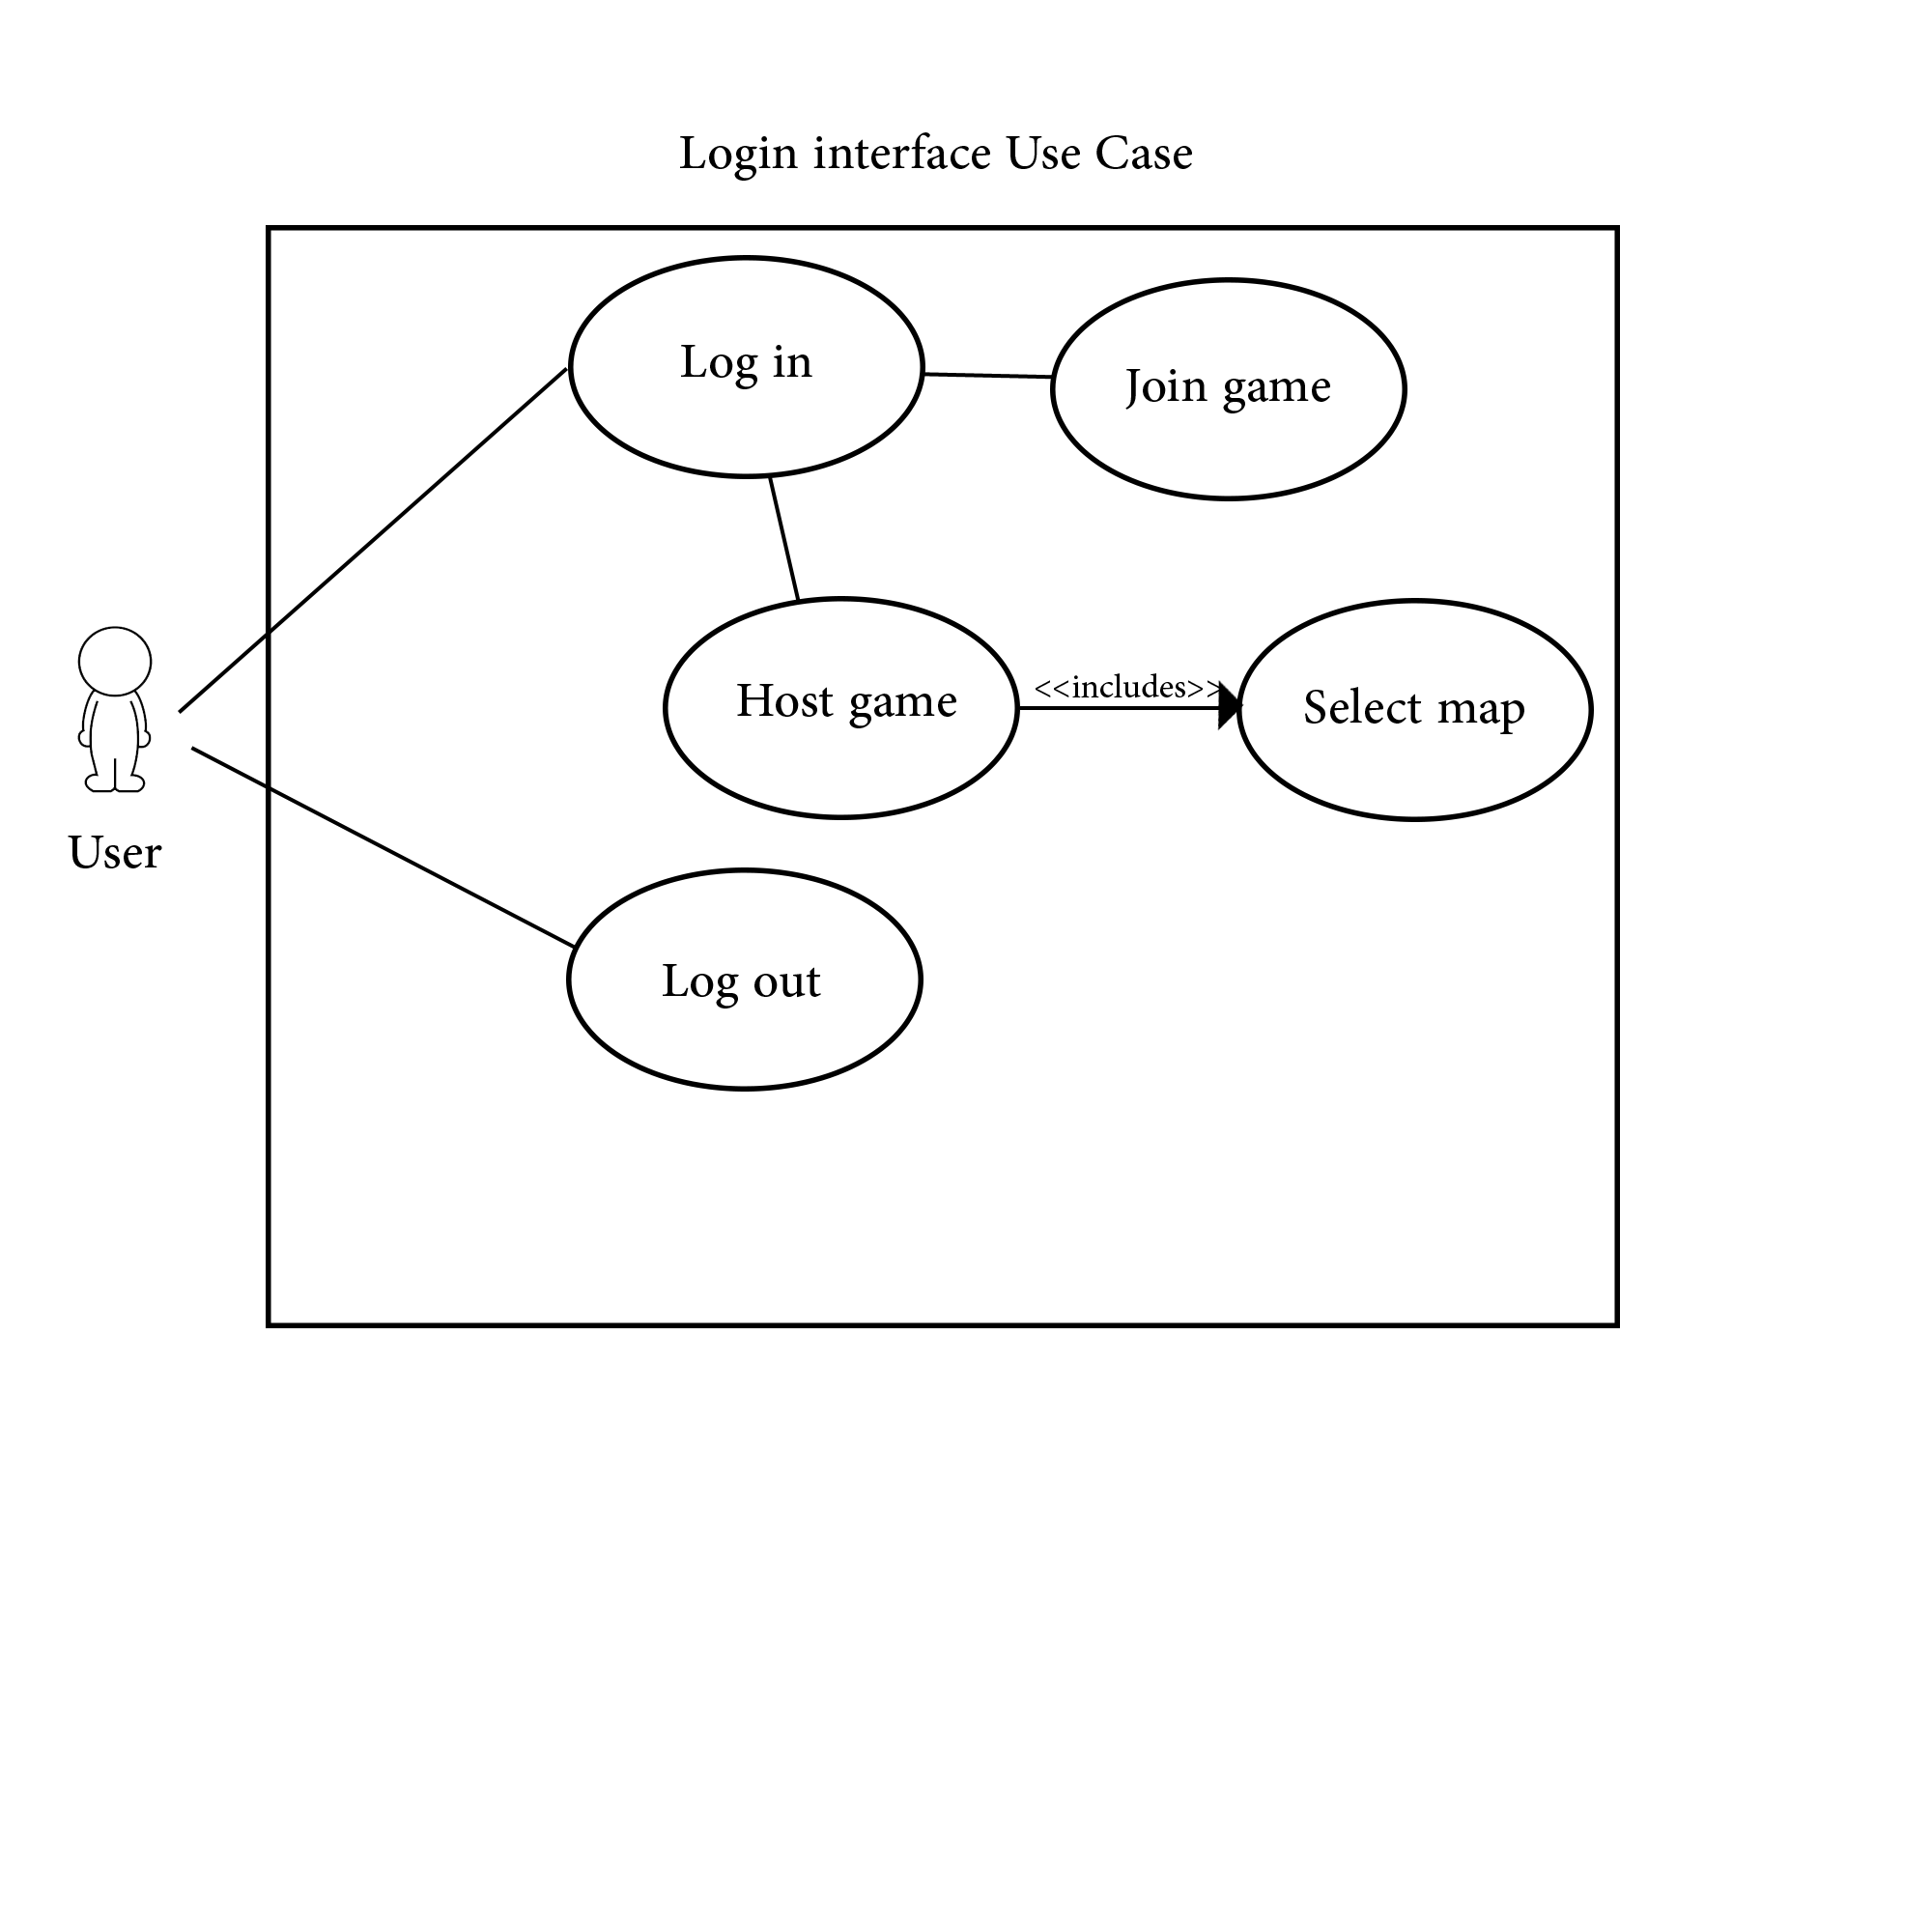
\includegraphics[width=500pt]{uml/useCaseDiagrams/loginUseCase.png}
    }
    \caption{Use Case Connection, Déconnection, Rejoindre Partie}
\end{figure}
\newpage
\subsubsection{Connection}
\paragraph{Préconditions}
\begin{itemize}
 \item Le jeu\index{jeu} doit être ouvert.
 \item L'utilisateur\index{utilisateur} ne doit pas être connecté.
\end{itemize}
\paragraph{Postconditions}
\begin{itemize}
 \item L'utilisateur\index{utilisateur} est connecté.
\end{itemize}
\paragraph{Cas général}
Une fois le jeu\index{jeu} démarrer, l'utilisateur\index{utilisateur} peut se connecté insérant un nom d'utilisateur existant et le mot de passe associé
[Exception : mauvais mot de passe ou pseudo\index{pseudo} non-existant].
Une fois toutes les informations entré, l'utilisateur\index{utilisateur} appuie sur le bouton \og \textit{Connect} \fg, et l'utilisateur\index{utilisateur} est
connecté. Un utilisateur\index{utilisateur} non-enregistré peut également créer un nouveau pseudo\index{pseudo} unique
et lui associé mot de passe en appuyant sur le bouton \og \textit{Create} \fg
[Exception: pseudo\index{pseudo} déjà utilisé].
Une fenêtre va ensuite s'ouvrir et lui demandé d'entrer les informations nécessaires 
[Exception: aucun pseudo\index{pseudo} et/ou mot de passe entré]. Ceci ajoutera sur le \textit{server} un nouvel utilisateur\index{utilisateur} avec comme
pseudo\index{pseudo} et mot de passe associés ceux entrés dans les zones appropriées, et connectera l'utilisateur\index{utilisateur} automatiquement.
\paragraph{Exceptions}
\begin{itemize}
 \item \textit{Mauvais mot de passe ou pseudo\index{pseudo} non-existant:} Après la pression du bouton \og \textit{Connect} \fg
 ,sur la même vue, une remarque apparait, en une couleur fortement
 perceptible, et indique à l'utilisateur\index{utilisateur} que les informations entrées sont incorrectes. La fenêtre de connexion reste ouverte et
 demande à l'utilisateur\index{utilisateur} de réentrer son pseudo\index{pseudo} et son mot de passe.
 \item \textit{Pseudo\index{pseudo} déja utilisé:} Après la pression du bouton \og \textit{Create} \fg,
 sur la même vue, une remarque apparait, en une couleur fortement
 perceptible, et indique à l'utilisateur\index{utilisateur} que le pseudo\index{pseudo} demandé est déjà utilisé. La fenêtre de création reste ouverte
 et demande à l'utilisateur\index{utilisateur} de réentrer un nouveau pseudo\index{pseudo}.
 \item \textit{Aucun pseudo\index{pseudo} et/ou mot de passe entré:} Dans les deux cas - de connexion ou de création - si l'utilisateur\index{utilisateur}
 manque d'entrer une information, après du bouton associé à la fenêtre en premier plan, sur la même vue,
 une remarque apparait, en une couleur fortement perceptible, et indique à l'utilisateur\index{utilisateur} l'information manquante. La
 fenêtre reste ouvert et demande à l'utilisateur\index{utilisateur} d'entrer cette information pour continuer la connexion ou la création.
\end{itemize}

\subsubsection{Déconnection}
\paragraph{Préconditions}
\begin{itemize}
 \item L'utilisateur\index{utilisateur} doit être connecté.
\end{itemize}
\paragraph{Postconditions}
\begin{itemize}
 \item L'utilisateur\index{utilisateur} est déconnecté.
 \item La fenêtre du jeu\index{jeu} est fermé.
\end{itemize}
\paragraph{Cas général}
Un joueur\index{joueur} peut se déconnecté à n'importe quel moment. Si il est en partie\index{partie}, il la quitte automatiquement. L'utilisateur\index{utilisateur}
est ensuite déconnecté et la fenêtre du jeu\index{jeu} se ferme.
\paragraph{Exceptions} Néant.
\subsubsection{Rejoindre Partie}
\paragraph{Préconditions}
\begin{itemize}
 \item L'utilisateur\index{utilisateur} est connecté.
\end{itemize}
\paragraph{Postconditions}
\begin{itemize}
 \item L'utilisateur\index{utilisateur} est dans une partie\index{partie}.
\end{itemize}
\paragraph{Cas général}
Un utilisateur\index{utilisateur} client peut rejoindre une partie\index{partie} en appuyant sur le bouton \og \textit{Join Game} \fg 
du menu principal.
Il est ensuite envoyé dans l'écran de sélection du jeu\index{jeu}, ou il lui est possible de voir toutes les parties\index{partie} lancées sur le
même \textit{serveur}\index{serveur} et visualiser les différentes informations sur chacune d'elles, comme le temps passé depuis le lancement
de la partie\index{partie} ou le status de celle-ci.
[Exception: la partie\index{partie} est complète]
Après avoir rejoins une partie\index{partie}, si celle-ci n'est pas commencé le joueur\index{joueur} est placé dans l’accueil où il peut
voir tous les joueurs\index{joueur} en attente - du début de la partie\index{partie} -, et la carte choisie. Il lui
est également possible de chatter avec les autres joueurs\index{joueur}. 
[Exception: Hôte ferme la partie\index{partie}]
Dans le cas où la partie\index{partie} est déjà commencé le joueur\index{joueur} reçoit de l'argent.
\paragraph{Exceptions}
\begin{itemize}
 \item \textit{La partie\index{partie} est complète:} Une fenêtre s'ouvre indiquant a l'utilisateur\index{utilisateur} que la partie\index{partie} est complète
 et donc injoignable. Une fois cette fenêtre fermée l'utilisateur\index{utilisateur} est ramené au menu de sélection.
 \item \textit{Hôte ferme la partie\index{partie}:} L'utilisateur\index{utilisateur} client est ramené au menu de sélection [pour plus d'informations, voir
 Host Game]. 
\end{itemize}

\subsubsection{Créer Partie}
\paragraph{Obligations spéciales}
\begin{itemize}
 \item Inclut Choisir Carte\index{carte}.
\end{itemize}
\paragraph{Préconditions}
\begin{itemize}
 \item L'utilisateur\index{utilisateur} doit être connecté.
\end{itemize}
\paragraph{Postconditions}
\begin{itemize}
 \item Une partie\index{partie} est ajoutée sur le \textit{serveur\index{serveur}}.
 \item Au moins 2 joueurs\index{joueur} participent.
\end{itemize}
\paragraph{Cas général}
L'utilisateur\index{utilisateur} est capable de créer une partie\index{partie} en appuyant sur le bouton \og \textit{Create game} \fg dans le menu principal.
Il choisit d'abords une carte\index{carte} et optionnellement d'autres options; la partie\index{partie} est alors créée, mais n'est pas lancée tant qu'il n'y a pas au moins 2 joueurs\index{joueur} qui participent.
Quand il y a assez de joueur\index{joueur} - minimum 2 et maximum 8 - le bouton \og \textit{Start game} \fg s'active. Quand il est cliqué, la partie\index{partie} démarre.
\paragraph{Exceptions} Néant.

\newpage
\subsubsection{Choisir Carte}
\paragraph{Obligations spéciales}
\begin{itemize}
 \item Est inclut dans Créer Partie.
\end{itemize}
\paragraph{Préconditions}
\begin{itemize}
 \item L'utilisateur\index{utilisateur} doit être dans le menu de création de partie\index{partie}.
\end{itemize}
\paragraph{Postconditions}
\begin{itemize}
 \item La carte choisie est chargée.
\end{itemize}
\paragraph{Cas général}
L'utilisateur\index{utilisateur} peut choisir une carte dans une liste prédéfinie de carte. Quand tous les éléments pour démarrer la partie\index{partie}
sont réunis [pour plus d'informations, voir Host Game], la carte est chargée.
\paragraph{Exceptions} Néant.

\newpage
\subsection{Achats libres}
\begin{figure}[ht]
    \makebox[\linewidth]{
        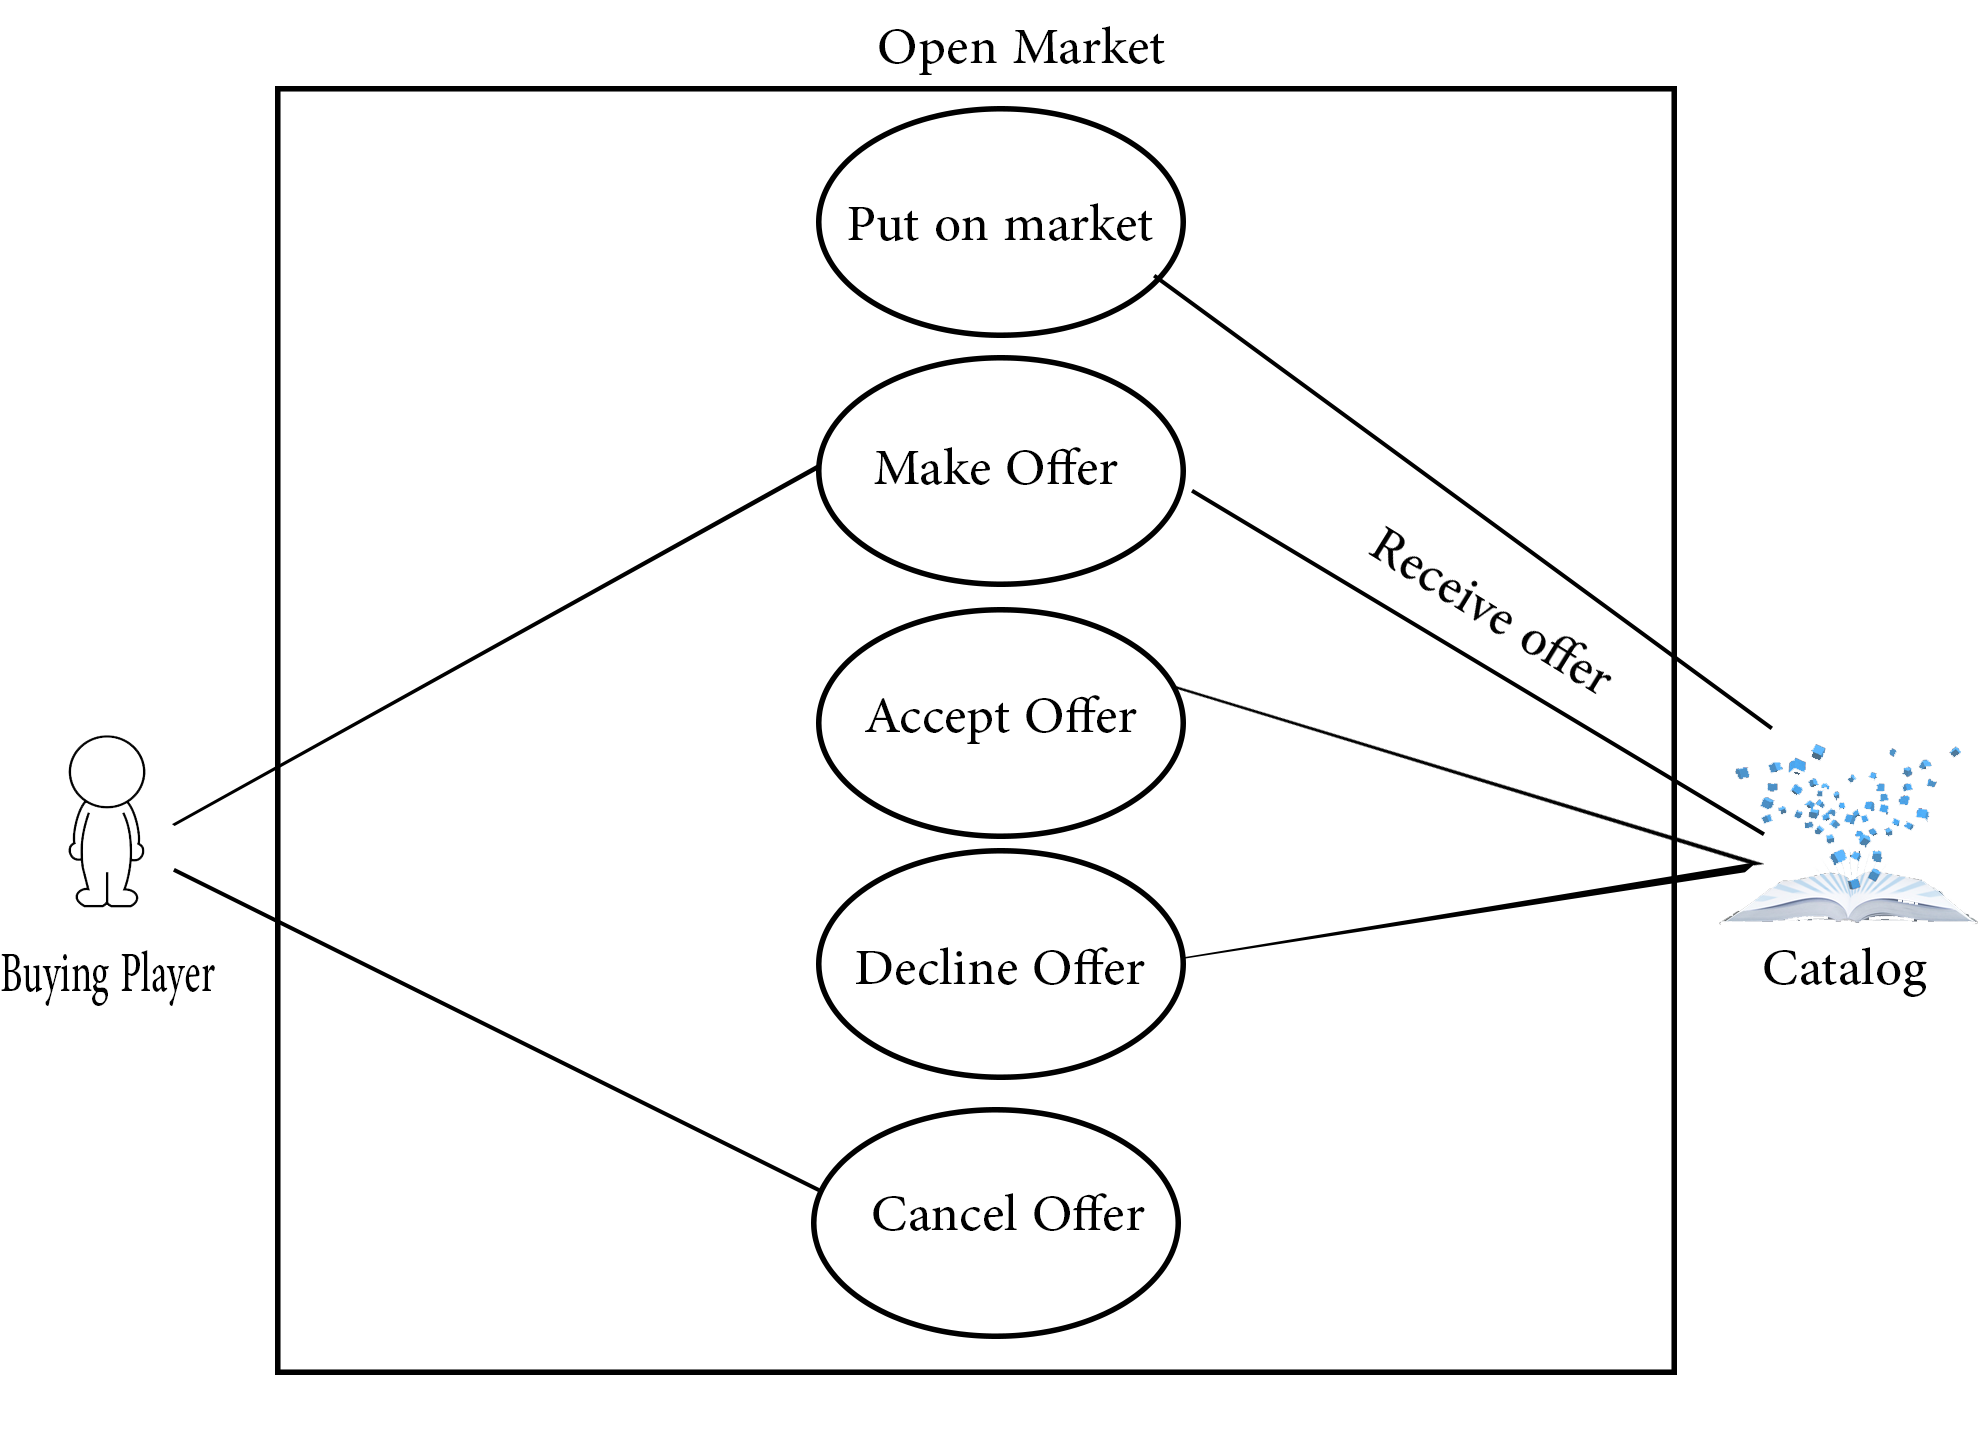
\includegraphics[width=500pt]{uml/useCaseDiagrams/buyUseCase.png}
    }
    \caption{Use Case Achats libres}
\end{figure}
\subsubsection{Faire une offre}
\paragraph{Préconditions}
\begin{itemize}
 \item La partie\index{partie} est en cours.
 \item La propriété voulue n'appartient à personne.
\end{itemize}
\paragraph{Postconditions}
\begin{itemize}
 \item Une offre pour une propriété est envoyée.
\end{itemize}
\paragraph{Cas général}
A tout moment de la partie\index{partie}, n'importe quel joueur\index{joueur} peut sélectionner une propriété dans le \textit{catalogue}\index{catalogue} qui n'a pas de propriétaire, et faire une offre sur celle-ci. Après avoir sélectionner la propriété, ses informations sont affichées, et le joueur\index{joueur} peut cliquer sur acheter.[Exception : Le joueur\index{joueur} n'a pas assez d'argent]
\paragraph{Exceptions}
\begin{itemize}
 \item \textit{Le joueur\index{joueur} n'a pas assez d'argent:} Une fenêtre s'ouvre indiquant au joueur\index{joueur} qu'il ne possède pas assez d'argent.
\end{itemize}

\subsubsection{Annuler une offre}
\paragraph{Préconditions}
\begin{itemize}
 \item La partie\index{partie} est en cours.
 \item Le joueur\index{joueur} à fait une offre qui n'as pas encore été validée.
\end{itemize}
\paragraph{Postconditions}
\begin{itemize}
 \item L'offre est annulée et retirée.
\end{itemize}
\paragraph{Cas général}
Dès que le joueur\index{joueur} a mit une offre et tant que celle-ci n'a pas été acceptée, ce joueur\index{joueur} peut annuler cette offre.
\paragraph{Exceptions} Néant.

\subsubsection{Accepter une offre}
\paragraph{Préconditions}
\begin{itemize}
 \item La partie\index{partie} est en cours.
 \item Un joueur\index{joueur} a fait une offre.
\end{itemize}
\paragraph{Postconditions}
\begin{itemize}
 \item Le joueur\index{joueur} paie le prix de la propriété.
 \item Le joueur\index{joueur} devient propriétaire de la propriété.
\end{itemize}
\paragraph{Cas général}
Lorsque le \textit{catalogue}\index{catalogue} reçoit une offre sur un bâtiment, il accepte automatiquement celle-ci.[Exception : Deux joueur\index{joueur} font la demande en même temps] Une fois l'offre acceptée, le joueur\index{joueur} doit confirmer son achat ou l'annuler.
\paragraph{Exceptions}
\begin{itemize}
 \item \textit{Deux joueur\index{joueur} font la demande en même temps:} La première offre reçue sera prise en compte, l'autre sera annulée.
\end{itemize}

\subsubsection{Mettre en vente}
\paragraph{Préconditions}
\begin{itemize}
 \item La partie\index{partie} est en cours.
 \item Il existe un bâtiment sans propriétaire.
\end{itemize}
\paragraph{Postconditions}
\begin{itemize}
 \item Le bâtiment est en vente libre.
\end{itemize}
\paragraph{Cas général}
Dès qu'un bâtiment n'as pas de prioritaire, le \textit{catalogue}\index{catalogue} le met en vente libre. Les bâtiments créés en début de partie\index{partie} seront mit dans le \textit{catalogue}\index{catalogue}, ainsi que les bâtiments d'un joueur\index{joueur} qui vient de perdre qui sont mit en vente libre.
\paragraph{Exceptions} Néant.

\newpage
\subsection{Construire-Améliorer-Détruire}
\begin{figure}[ht]
    \makebox[\linewidth]{
        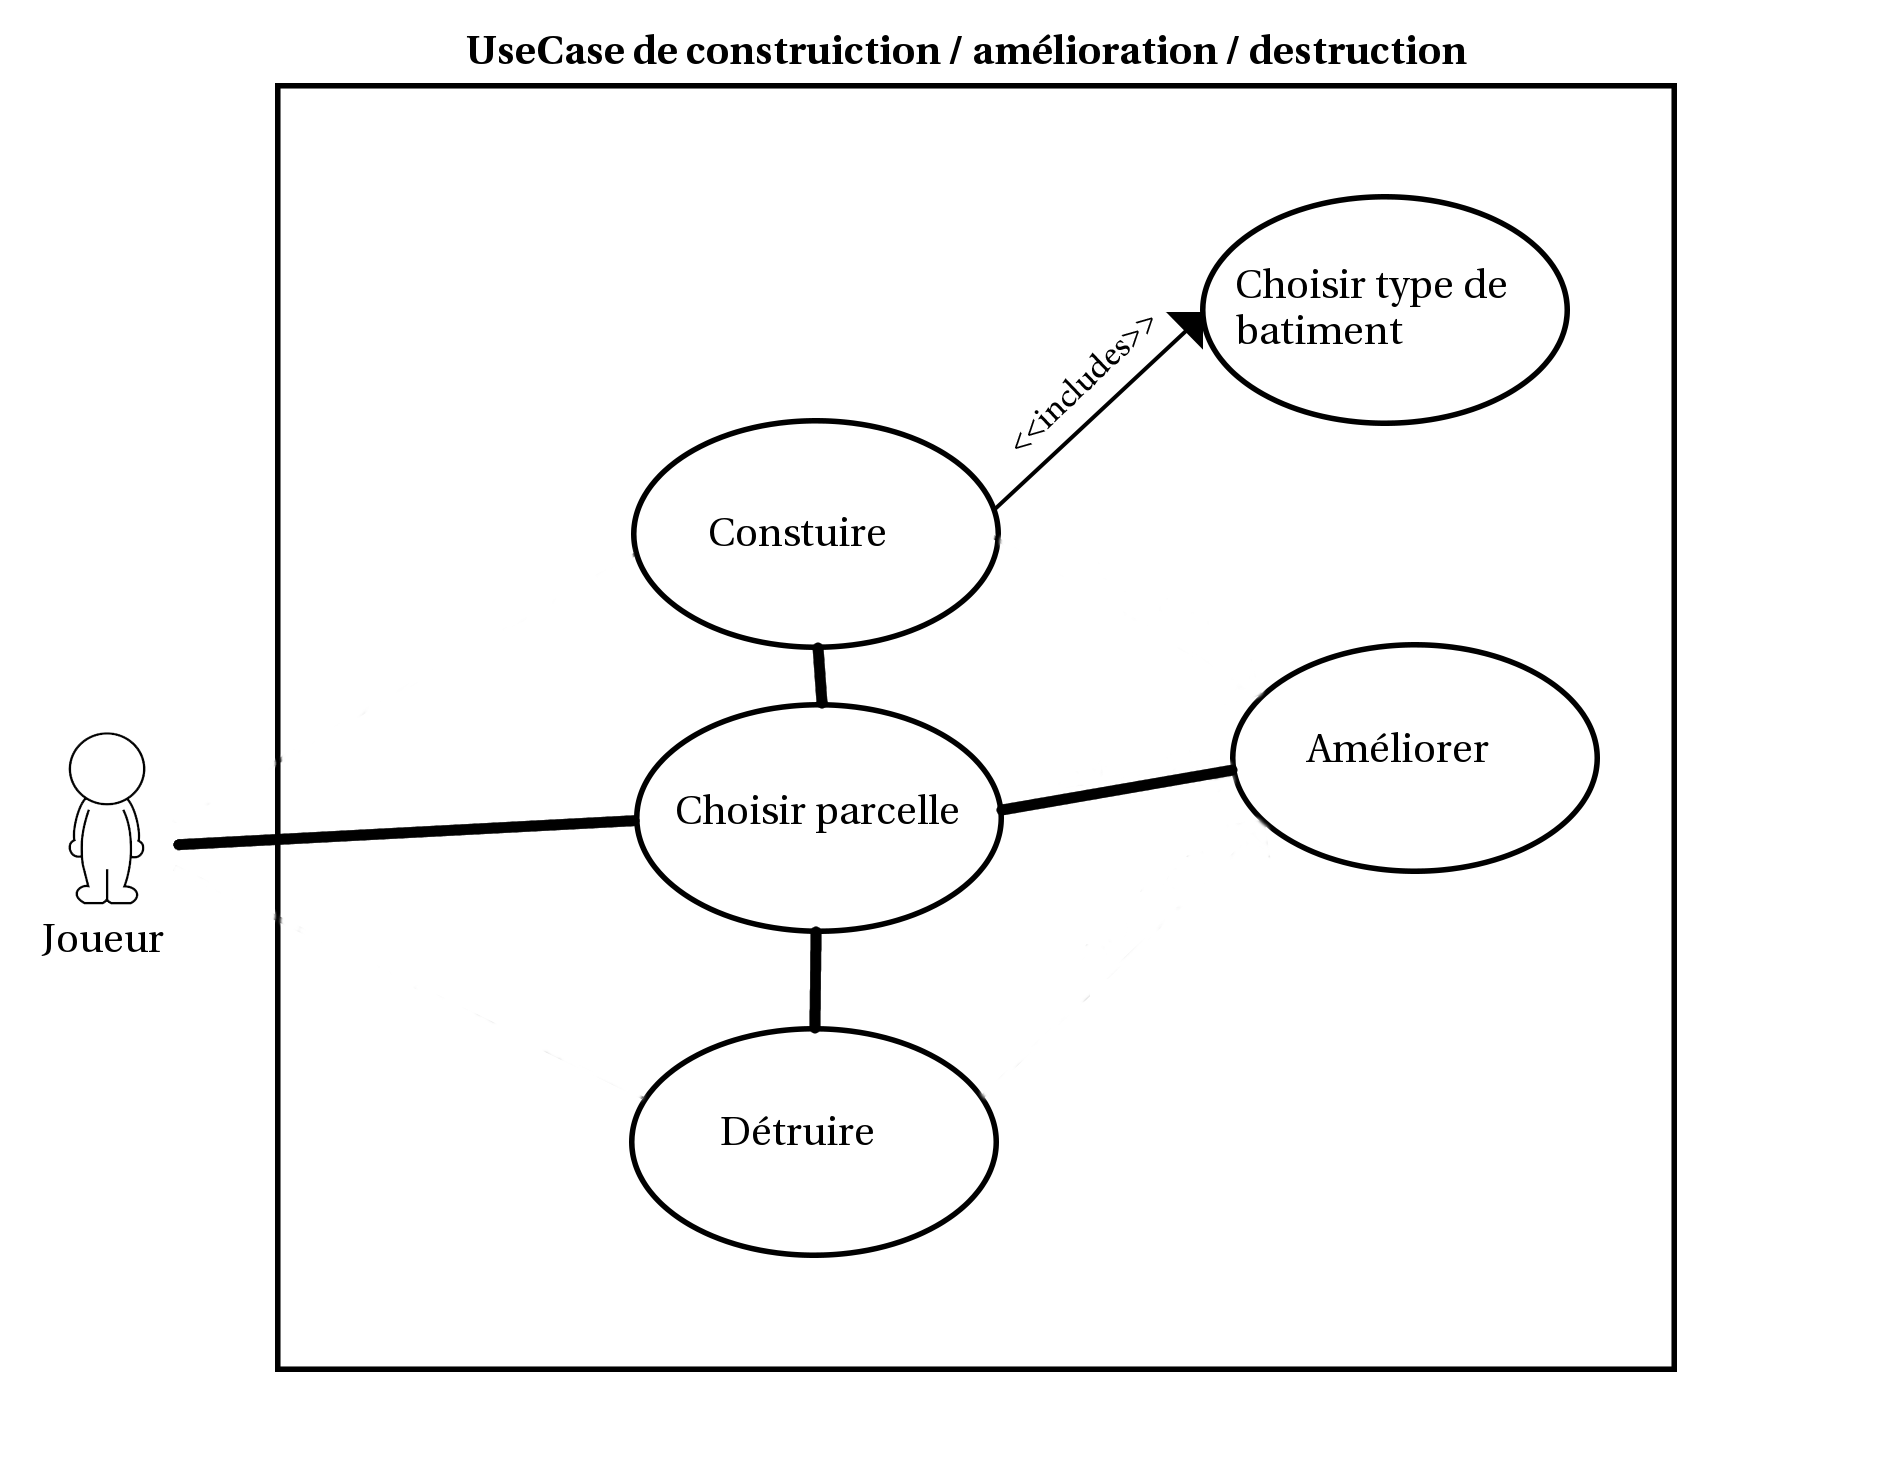
\includegraphics[width=550pt]{uml/useCaseDiagrams/buildDestroyUseCase.png}
    }
    \caption{Use Case Buid/Upgrade/Destroy}
\end{figure}

\subsubsection{Choisir lieu}
\paragraph{Préconditions}
\begin{itemize}
	\item Le joueur\index{joueur} est dans une partie\index{partie}, sur l'écran de jeu\index{jeu}.
\end{itemize}
\paragraph{Postconditions}
\begin{itemize}
	\item Une propriété est sélectionnée.
	\item Les informations sur cette propriété sont affichées.
	\item Les boutons <Buy>,<Build>,<Upgrade>,<Sell>,<Demolish> s'activent ou se désactivent selon la propriété sélectionnée.
\end{itemize}
\paragraph{Cas général}
Le joueur\index{joueur} doit simplement cliquer, sur la carte, sur le terrain exigé.[Exception : Sélection invalide]
\paragraph{Exceptions}
\begin{itemize}
	\item \textit{Sélection invalide:} Si l'emplacement sélectionné n'est pas un terrain/bâtiment (et donc une route ou un obstacle), la sélection n'est pas faite.
\end{itemize}

\subsubsection{Construire}
\paragraph{Obligations spéciales}
\begin{itemize}
 \item Inclut Choisir type de Bâtiment.
\end{itemize}
\paragraph{Préconditions}
\begin{itemize}
 \item La partie\index{partie} est en cours.
 \item Le joueur\index{joueur} a sélectionné une parcelle qui lui appartient et est vide. (Le bouton <Build> est activé).
\end{itemize}
\paragraph{Postconditions}
\begin{itemize}
 \item Un bâtiment est construit et affiché sur la carte.
 \item Le joueur\index{joueur} possède ce nouveau bâtiment.
 \item Le joueur\index{joueur} a payé le prix de construction.
\end{itemize}
\paragraph{Cas général}
Lorsque un joueur\index{joueur} veut construire un nouveau bâtiment, il lui faudra simplement sélectionner une parcelle qui lui appartient et est vide. Le bouton \og \textit{<Build>} \fg s'activera. Le joueur\index{joueur} devra cliquer dessus, il entre alors en mode Construction; Un tableau s'affichera, permettant au joueur\index{joueur} de sélection un type de bâtiment et affichant les informations sur ce type. Il peut à tout moment quitter ce mode et annuler la construction, en cliquant sur \og \textit{Annuler} \fg. Pour valider l'opération, le joueur\index{joueur} cliquera sur \og \textit{<Ok>} \fg.[Exception : Le joueur\index{joueur} n'as pas assez d'argent] Il devra payer ensuite le prix indiqué.
\paragraph{Exceptions}
\begin{itemize}
 \item \textit{Le joueur\index{joueur} n'as pas assez d'argent:}  Une fenêtre s'ouvre indiquant au joueur\index{joueur} qu'il ne possède pas assez d'argent.
\end{itemize}
\subsubsection{Améliorer}\index{améliorer}
\paragraph{Préconditions}
\begin{itemize}
 \item La partie\index{partie} est en cours.
 \item Le joueur\index{joueur} possède au moins un bâtiment.
 \item Le joueur\index{joueur} a sélectionné une parcelle qui lui appartient et qui a un bâtiment améliorable. (Le bouton <Upgrade> est activé).
\end{itemize}
\paragraph{Postconditions}
\begin{itemize}
 \item Un bâtiment sélectionné est amélioré d'un niveau.
 \item Le joueur\index{joueur} a dépensé de l'argent pour l'amélioration.
\end{itemize}
\paragraph{Cas général}
Lorsque un joueur\index{joueur} veut améliorer\index{améliorer} un bâtiment, il lui faudra simplement sélectionner une parcelle qui lui appartient et qui possède un bâtiment améliorable. Le bouton \og \textit{<Upgrade>} \fg s'activera. Le joueur\index{joueur} devra cliquer dessus. Un tableau s'affichera, permettant au joueur\index{joueur} de voir les informations sur le niveau supérieur de ce bâtiment.[Exception : Bâtiment amélioré au max] Pour valider l'opération, le joueur\index{joueur} cliquera sur \og \textit{<Ok>} \fg.[Exception : Le joueur\index{joueur} n'as pas assez d'argent] Il devra payer ensuite le prix indiqué.
\paragraph{Exceptions}
\begin{itemize}
 \item \textit{Le joueur\index{joueur} n'as pas assez d'argent:}  Une e s'ouvre indiquant au joueur\index{joueur} qu'il ne possède pas assez d'argent.
 \item \textit{Bâtiment amélioré au max:}  Les bâtiments ont un niveau maximum d'amélioration Une fenêtre s'ouvre indiquant au joueur\index{joueur} qu'il ne peut plus améliorer ce bâtiment.
\end{itemize}
\subsubsection{Détruire}
\paragraph{Préconditions}
\begin{itemize}
 \item La partie\index{partie} est en cours.
 \item Le joueur\index{joueur} possède au moins un bâtiment.
 \item Le joueur\index{joueur} a sélectionné une parcelle qui lui appartient et qui a un bâtiment. (Le bouton <Destroy> est activé).
\end{itemize}
\paragraph{Postconditions}
\begin{itemize}
 \item Un bâtiment est détruit et n’existe plus.
 \item Le propriétaire gagne une somme d'argent équivalente à la moitié de la valeur du bâtiment détruit.
\end{itemize}
\paragraph{Cas général}
Un joueur\index{joueur} peut également détruire un de ses bâtiments. Il lui suffit de sélectionner une parcelle qui lui appartient et qui possède un bâtiment et ensuite de cliquer sur le bouton \og \textit{<Destroy>} \fg. Un tableau s'affichera montrant le gain de la destruction. Il peut à tout moment quitter ce mode et annuler la destruction en cliquant sur \og \textit{<Annuler>} \fg. Pour valider l'opération, le joueur\index{joueur} cliquera sur \og \textit{<Ok>} \fg. Une fois détruit, le bâtiment rapporte la moitié de la valeur de celui-ci à son propriétaire.
\newpage
\subsubsection{Choisir type de Bâtiment}
\paragraph{Obligations spéciales}
\begin{itemize}
 \item Est inclut dans construire.
\end{itemize}
\paragraph{Préconditions}
\begin{itemize}
 \item Le joueur\index{joueur} est entré en mode Construction.
\end{itemize}
\paragraph{Postconditions}
\begin{itemize}
 \item Un type est sélectionné pour la construction.
 \item Les information lié à ce type sont affiché dans le tableau de construction.
\end{itemize}
\paragraph{Cas général}
Un \textit{catalogue}\index{catalogue} de types prédéfinis de bâtiment(bar,magasin,night-club,...) apparaît, pour chaque type les statistiques (prix, coûts, capacité, heures,..) sont affichés. Il suffit au joueur\index{joueur} alors de cliquer sur le type désiré.
\paragraph{Exceptions} Néant.



\newpage
\subsection{Achats entre joueurs}\index{joueur}
\begin{figure}[ht]
    \makebox[\linewidth]{
        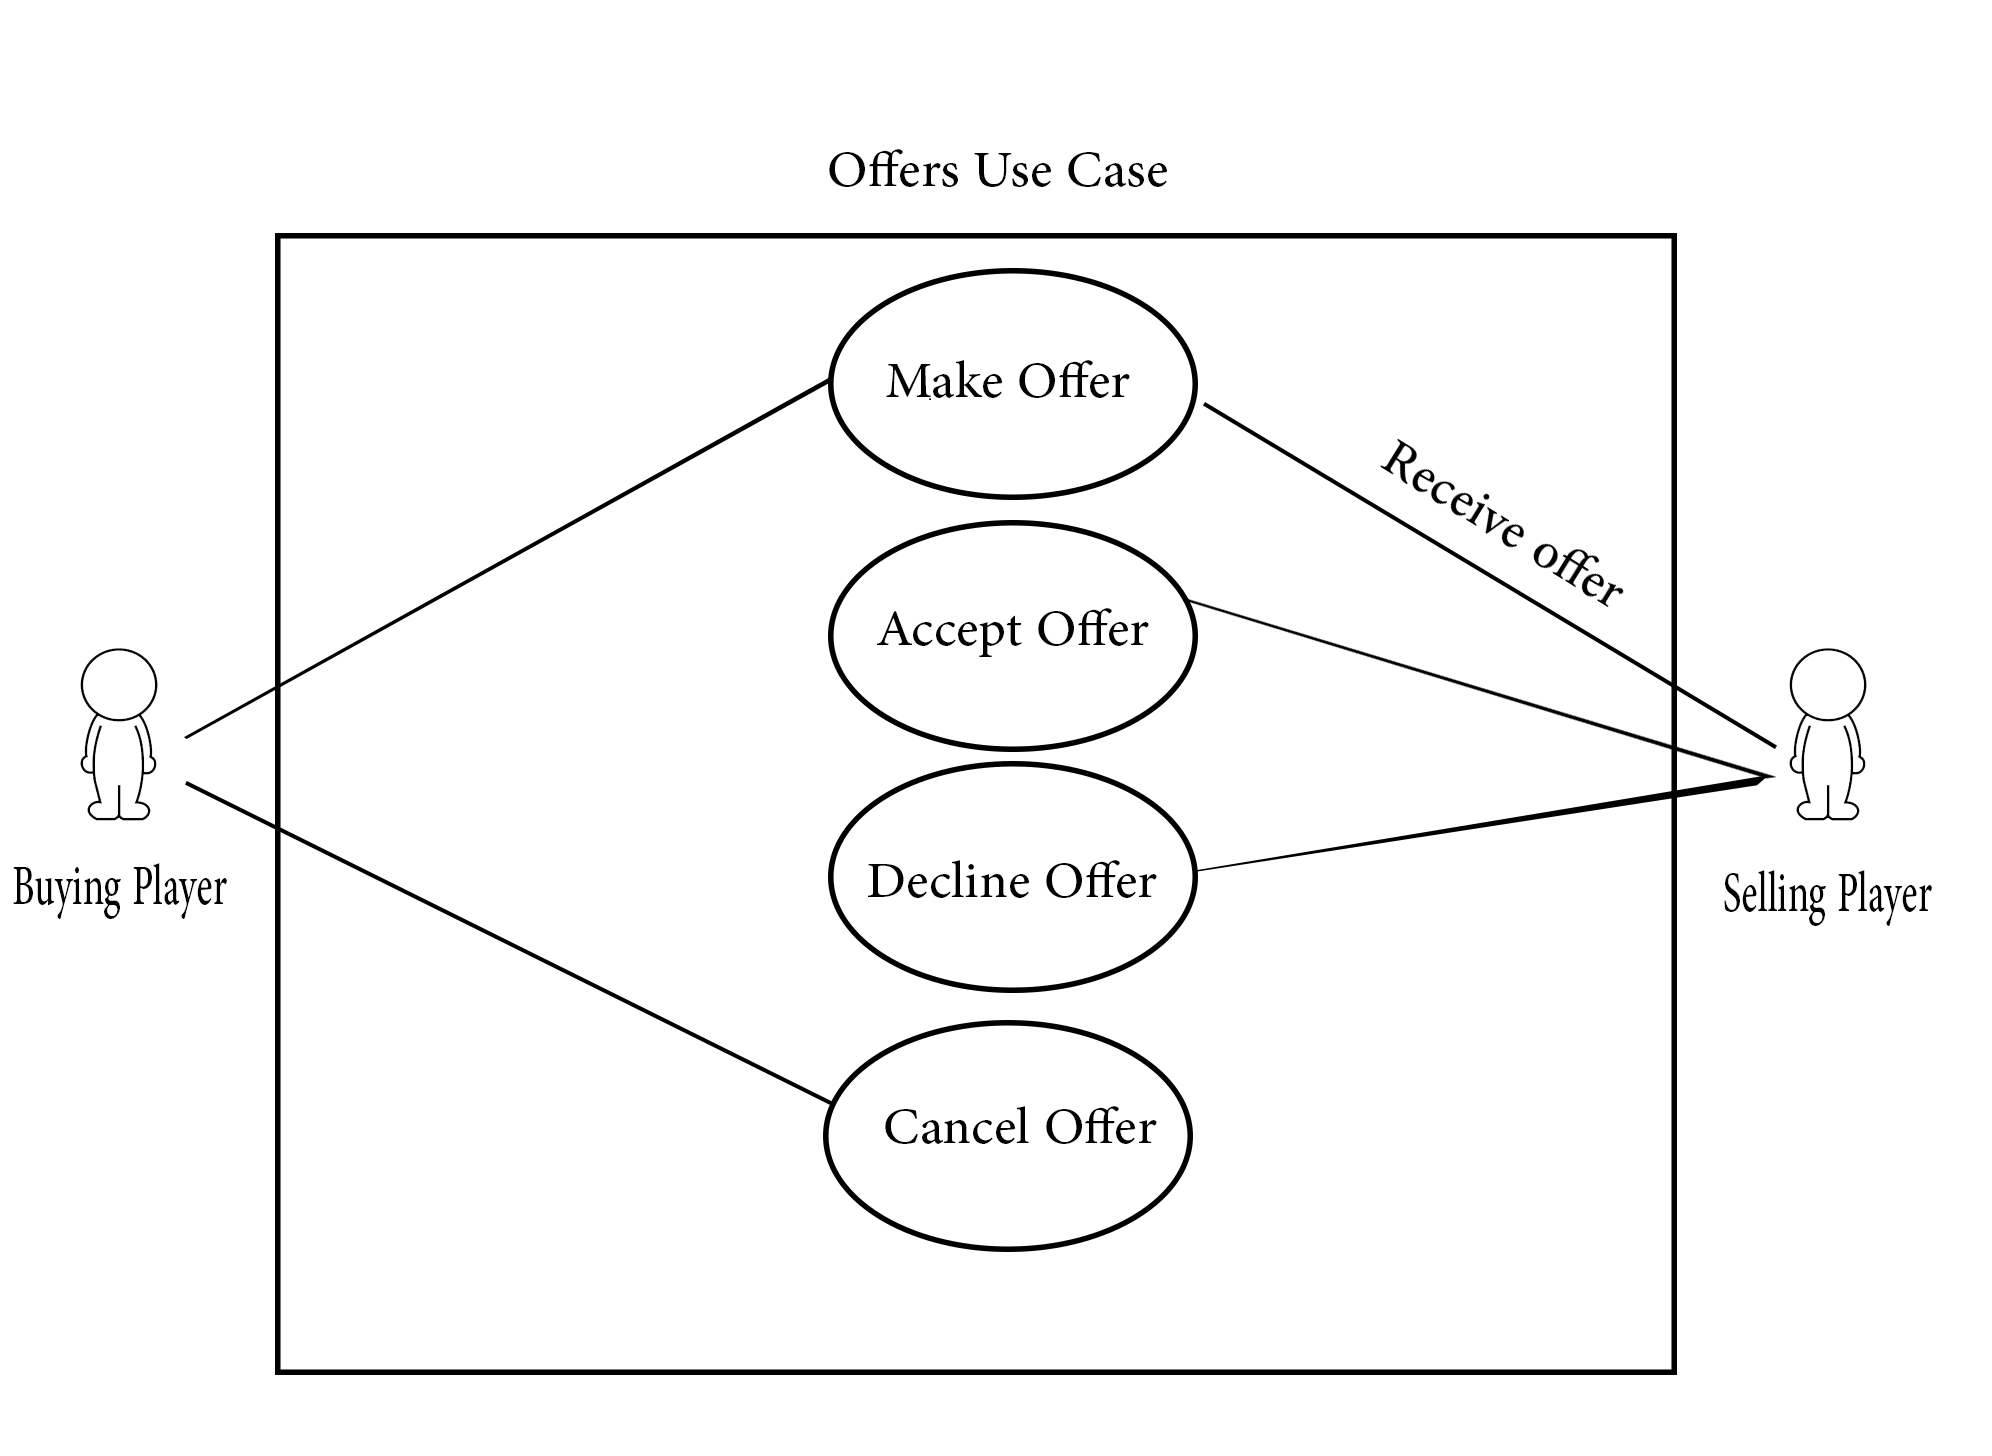
\includegraphics[width=550pt]{uml/useCaseDiagrams/offerUseCase.png}
    }
    \caption{Use Case Achats entre joueurs}
\end{figure}
\subsubsection{Faire une offre}
\paragraph{Préconditions}
\begin{itemize}
 \item La partie\index{partie} est en cours.
 \item La propriété voulue appartient à un joueur\index{joueur}.
\end{itemize}
\paragraph{Postconditions}
\begin{itemize}
 \item Une offre pour une propriété est envoyé à un autre joueur\index{joueur}.
\end{itemize}
\paragraph{Cas général}
A tout moment de la partie\index{partie}, un joueur\index{joueur} peut tenter d'acheter le bâtiment d'un autre. Il lui doit simplement de faire une offre auprès de ce joueur\index{joueur}, pour ce bâtiment.[Exception : Le joueur\index{joueur} a fait trop d'offre] Il suffit à l'acheteur de sélectionner le bâtiment voulu et de cliquer sur \og \textit{Faire une offre} \fg, une fenêtre s'ouvre pour que le joueur\index{joueur} puisse donner le prix qu'il est prêt a payer et confirme son offre.[Exception : Le joueur\index{joueur} n'a pas assez d'argent] 
\paragraph{Exceptions}
\begin{itemize}
 \item \textit{Le joueur\index{joueur} n'a pas assez d'argent:} Une fenêtre s'ouvre indiquant au joueur\index{joueur} qu'il ne possède pas assez d'argent.
 \item \textit{Le joueur\index{joueur} a fait trop d'offre:} Afin d'éviter tout spam, une limite d'offre sur un temps donné est instauré.
\end{itemize}
\subsubsection{Annuler une offre}
\paragraph{Préconditions}
\begin{itemize}
 \item La partie\index{partie} est en cours.
 \item Le joueur\index{joueur} à fait une offre qui n'a pas encore été validée.
\end{itemize}
\paragraph{Postconditions}
\begin{itemize}
 \item L'offre est annulée.
\end{itemize}
\paragraph{Cas général}
Dès que le joueur\index{joueur} a mit une offre et tant que celle-ci n'a pas été acceptée, ce joueur\index{joueur} peut annuler cette offre.
\paragraph{Exceptions} Néant.
\subsubsection{Accepter une offre}
\paragraph{Préconditions}
\begin{itemize}
 \item La partie\index{partie} est en cours.
 \item Un joueur\index{joueur} a reçu une offre.
\end{itemize}
\paragraph{Postconditions}
\begin{itemize}
 \item L'acheteur devient propriétaire de la propriété.
 \item Le vendeur reçoit une compensation monétaire et perd sa propriété.
\end{itemize}
\paragraph{Cas général}
Lorsque un joueur\index{joueur} reçoit une offre sur un bâtiment, une fenêtre s'affiche avec les informations sur cette offre, il peut accepter celle-ci en cliquant sur \og \textit{Accepter} \fg.
\paragraph{Exceptions} Néant
\subsubsection{Refuser une offre}
\paragraph{Préconditions}
\begin{itemize}
 \item La partie\index{partie} est en cours.
 \item Un joueur\index{joueur} a reçu une offre.
\end{itemize}
\paragraph{Postconditions}
\begin{itemize}
 \item L'offre est annulée.
\end{itemize}
\paragraph{Cas général}
Lorsque un joueur\index{joueur} reçoit une offre sur un bâtiment, une fenêtre s'affiche avec les informations sur cette offre, il peut refuser celle-ci en cliquant sur \og \textit{Refuser} \fg.
\paragraph{Exceptions} Néant


\newpage
\subsection{Sabotage}
\begin{figure}[ht]
	\makebox[\linewidth]{
		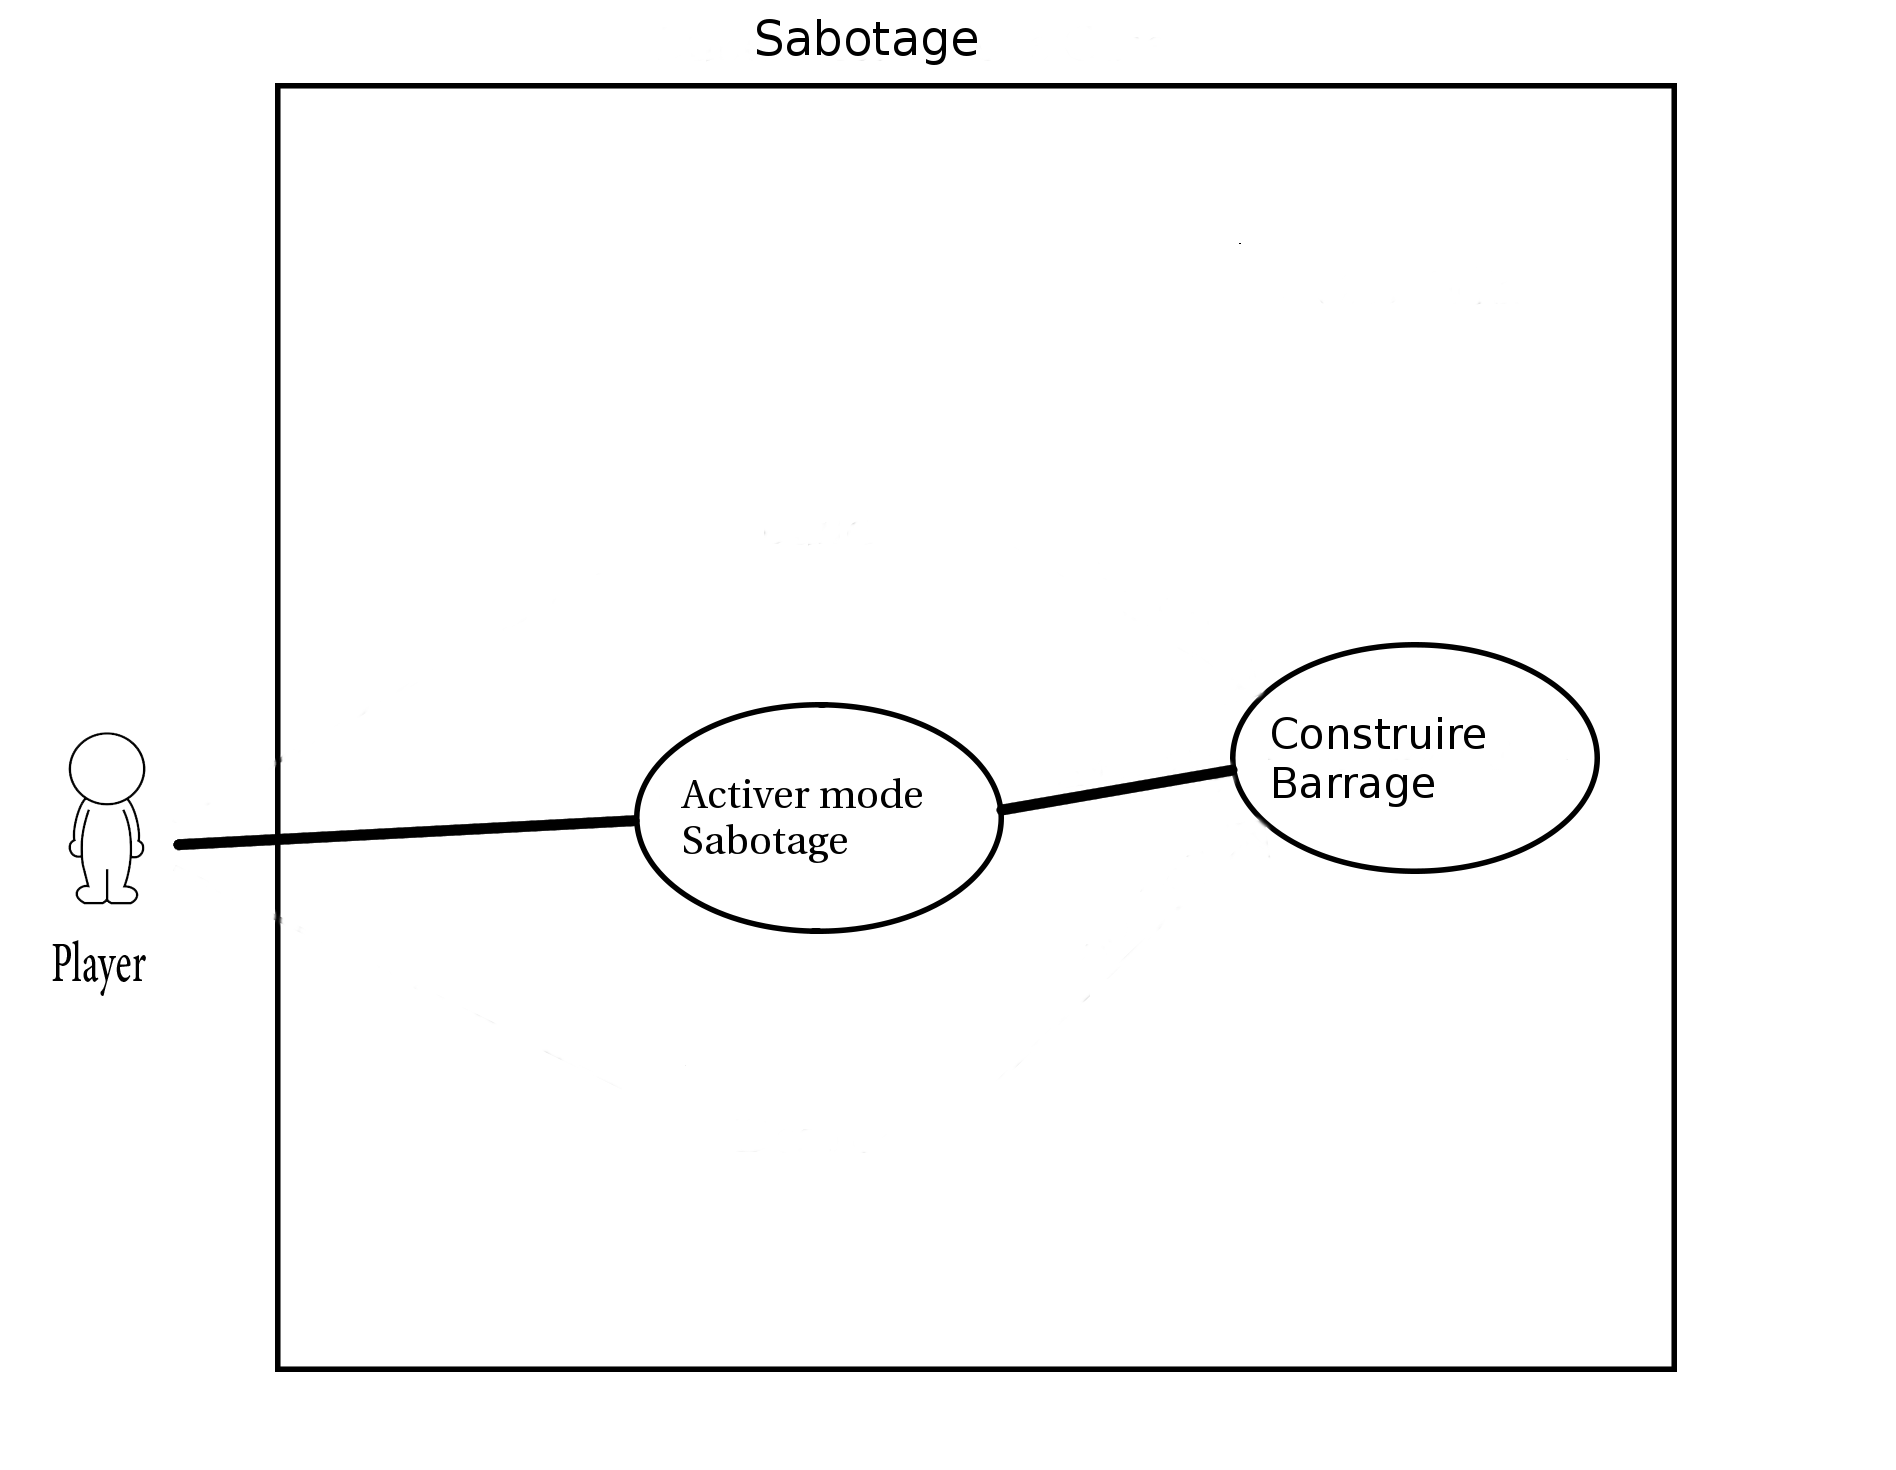
\includegraphics[width=550pt]{uml/useCaseDiagrams/sabotage.png}
	}
	\caption{Use Case Buid/Upgrade/Destroy}
\end{figure}

\subsubsection{Choisir Lieu}
\paragraph{Préconditions}
\begin{itemize}
	\item Le joueur\index{joueur} est dans une partie\index{partie}, sur l'écran de jeu\index{jeu}.
\end{itemize}
\paragraph{Postconditions}
\begin{itemize}
	\item Une propriété est sélectionnée.
	\item Les informations sur cette propriété sont affichées.
	\item Les boutons <Buy>,<Build>,<Upgrade>,<Sell>,<Demolish> s'activent ou se désactivent selon la propriété sélectionnée.
\end{itemize}
\paragraph{Cas général}
Le joueur\index{joueur} doit simplement cliquer, sur la carte, sur le terrain exigé.[Exception : Sélection invalide]
\paragraph{Exceptions}
\begin{itemize}
	\item \textit{Sélection invalide:} Si l'emplacement sélectionné n'est pas un terrain/bâtiment (et donc une route ou un obstacle), la sélection n'est pas faite.
\end{itemize}

\subsubsection{Construire Barrage}
\paragraph{Préconditions}
\begin{itemize}
	\item La partie\index{partie} est en cours.
	\item Le joueur\index{joueur} a sélectionné une route qui est vide.
\end{itemize}
\paragraph{Postconditions}
\begin{itemize}
	\item Un barrage est construit et affiché sur la carte à l'emplacement séléctionné.
	\item Le joueur\index{joueur} a payé le prix de construction du barrage.
\end{itemize}
\paragraph{Cas général}
Lorsque un joueur\index{joueur} veut construire un nouveau barrage, il lui faudra simplement sélectionner une route est vide. Le bouton \og \textit{<Build RoadBlock>} \fg s'activera. Le joueur\index{joueur} devra cliquer dessus, il entre alors en mode Construction; Un tableau s'affichera affichant les informations sur le barrage. Il peut à tout moment quitter ce mode et annuler la construction, en cliquant sur \og \textit{Annuler} \fg. Pour valider l'opération, le joueur\index{joueur} cliquera sur \og \textit{<Ok>} \fg.[Exception : Le joueur\index{joueur} n'as pas assez d'argent] Il devra payer ensuite le prix indiqué.
\paragraph{Exceptions}
\begin{itemize}
	\item \textit{Le joueur\index{joueur} n'as pas assez d'argent:}  Une fenêtre s'ouvre indiquant au joueur\index{joueur} qu'il ne possède pas assez d'argent.
\end{itemize}




\newpage
\section{Exigences non fonctionnelles}
\subsection{Service}
\paragraph{}Ergonomie:  \newline
Le \textit{système}\index{système} sera crée de telle sorte qu'il disposera d’une apparence graphique concise, afin que le joueur\index{joueur} puisse repérer les options dont il a besoin dans le menu du jeu\index{jeu}.

La map sera aura comme particularité que chaque joueur\index{joueur} aura sa couleur qui sera affichée sur ses propriétés.

L'utilisation sera facilitée par l'interface graphique, grâce à des icônes, boutons et aides affichées tout au long du jeu\index{jeu}.

\paragraph{}Aptitude à la maintenance:  \newline
Le concept de programmation orientée objet étant suivit avec rigueur pour l’implémentation du jeu\index{jeu}, celui-ci permettra la mise à jour ou le débuggage du jeu\index{jeu}.

\paragraph{}Compatibilité:  \newline
Le jeu\index{jeu} est implémenté sur et pour un \textit{système}\index{système} d'exploitation Linux seulement.

\paragraph{}Rétablissement:  \newline
Dans le cas d'un crash ou d'arrêt de \textit{serveur}\index{serveur}, il faut faire en sorte que les joueurs\index{joueur} puissent reprendre leur partie\index{partie}. Le \textit{serveur}\index{serveur} fera donc une sauvegarde automatique à chaque debut de journée(de la partie\index{partie} en cours, 7h du matin). 
Vu qu'une seule sauvegarde est nécessaire, la nouvelle remplacera la précédente.
Si la partie\index{partie} se termine, la sauvegarde lié à celle-ci sera supprimée.

Quand le \textit{serveur}\index{serveur} re-démarre, il vérifie si une partie\index{partie} en cours a été interrompue; si oui, il relance la partie\index{partie} grâce à sa sauvegarde.

\paragraph{}Disponibilité:  \newline
Le jeu\index{jeu} sera disponible 24h/24 7j/7, tant que le serveur\index{serveur} tourne. Celui ne sera arrêté que brièvement lors de possible maintenance de débuggage\index{débug} et mise à jour.

\subsection{Contraintes}
\paragraph{}
Afin de fonctionner correctement, et d’avoir une expérience de jeu\index{jeu} optimale, le \textit{système}\index{système} devra être lancé sur un ordinateur possédant la configuration nécessaire.
En cas d’environnement peu performant, il est possible que des ralentissements, ou qu’un manque de fluidité se fasse ressentir.
\paragraph{}
Il est également nécessaire que le \textit{système}\index{système} soit accompagné d’une connexion internet stable et rapide.
Sans cela, la communication avec le \textit{serveur}\index{serveur} et entre les joueurs\index{joueur} serait endommagée, et endommagerait la jouabilité de tous les joueurs\index{joueur}.

\newpage

\section{Exigences de domaine}
\begin{itemize}
 \item Le jeu\index{jeu} est multi-joueur\index{multi-joueur}, et doit donc permettre aux différents utilisateurs\index{utilisateur} de communiquer entre eux.
 \item Une partie\index{partie} doit être composé d'au minimum 2 joueurs\index{joueur} et au maximum 8 joueurs\index{joueur}.
 \item Les 8 premiers joueurs\index{joueur} qui rejoignent la partie\index{partie} seront les seules 8 joueurs\index{joueur} capable de la rejoindre.
 \item Pour qu'un joueur\index{joueur} puisse continuer à jouer, il doit posséder soit des terrains, des batiments ou encore avoir
 un capital. 
 \item Le capitale de chaque joueur\index{joueur} varie tout au long de la partie\index{partie} en fonction des frais et des gains de chaque bâtiment.
 \item Les gains qu'apporte chaque bâtiment seront représentés par des visiteurs, qui, en suivant un chemin, pourront 
 rentrer dans un bâtiment qui augmentera le capital de son propriétaire.
 \item Si le joueur\index{joueur} est en faillite, la partie\index{partie} se terminera pour ce joueur\index{joueur} et il ne sera plus possible pour lui de
 continuer de jouer dans cette partie\index{partie}, mais il pourra toute fois la regarder.
 \item La partie\index{partie} se finie uniquement si il ne reste plus qu'un joueur\index{joueur} propriétaire.

 \end{itemize}

\newpage
\chapter{Besoins du système}\index{système}
\section{Exigences fonctionnelles}
\section{Exigences non fonctionnelles}
\section{Design et fonctionnement du système}\index{système}
\begin{figure}[ht]
    \makebox[\linewidth]{
        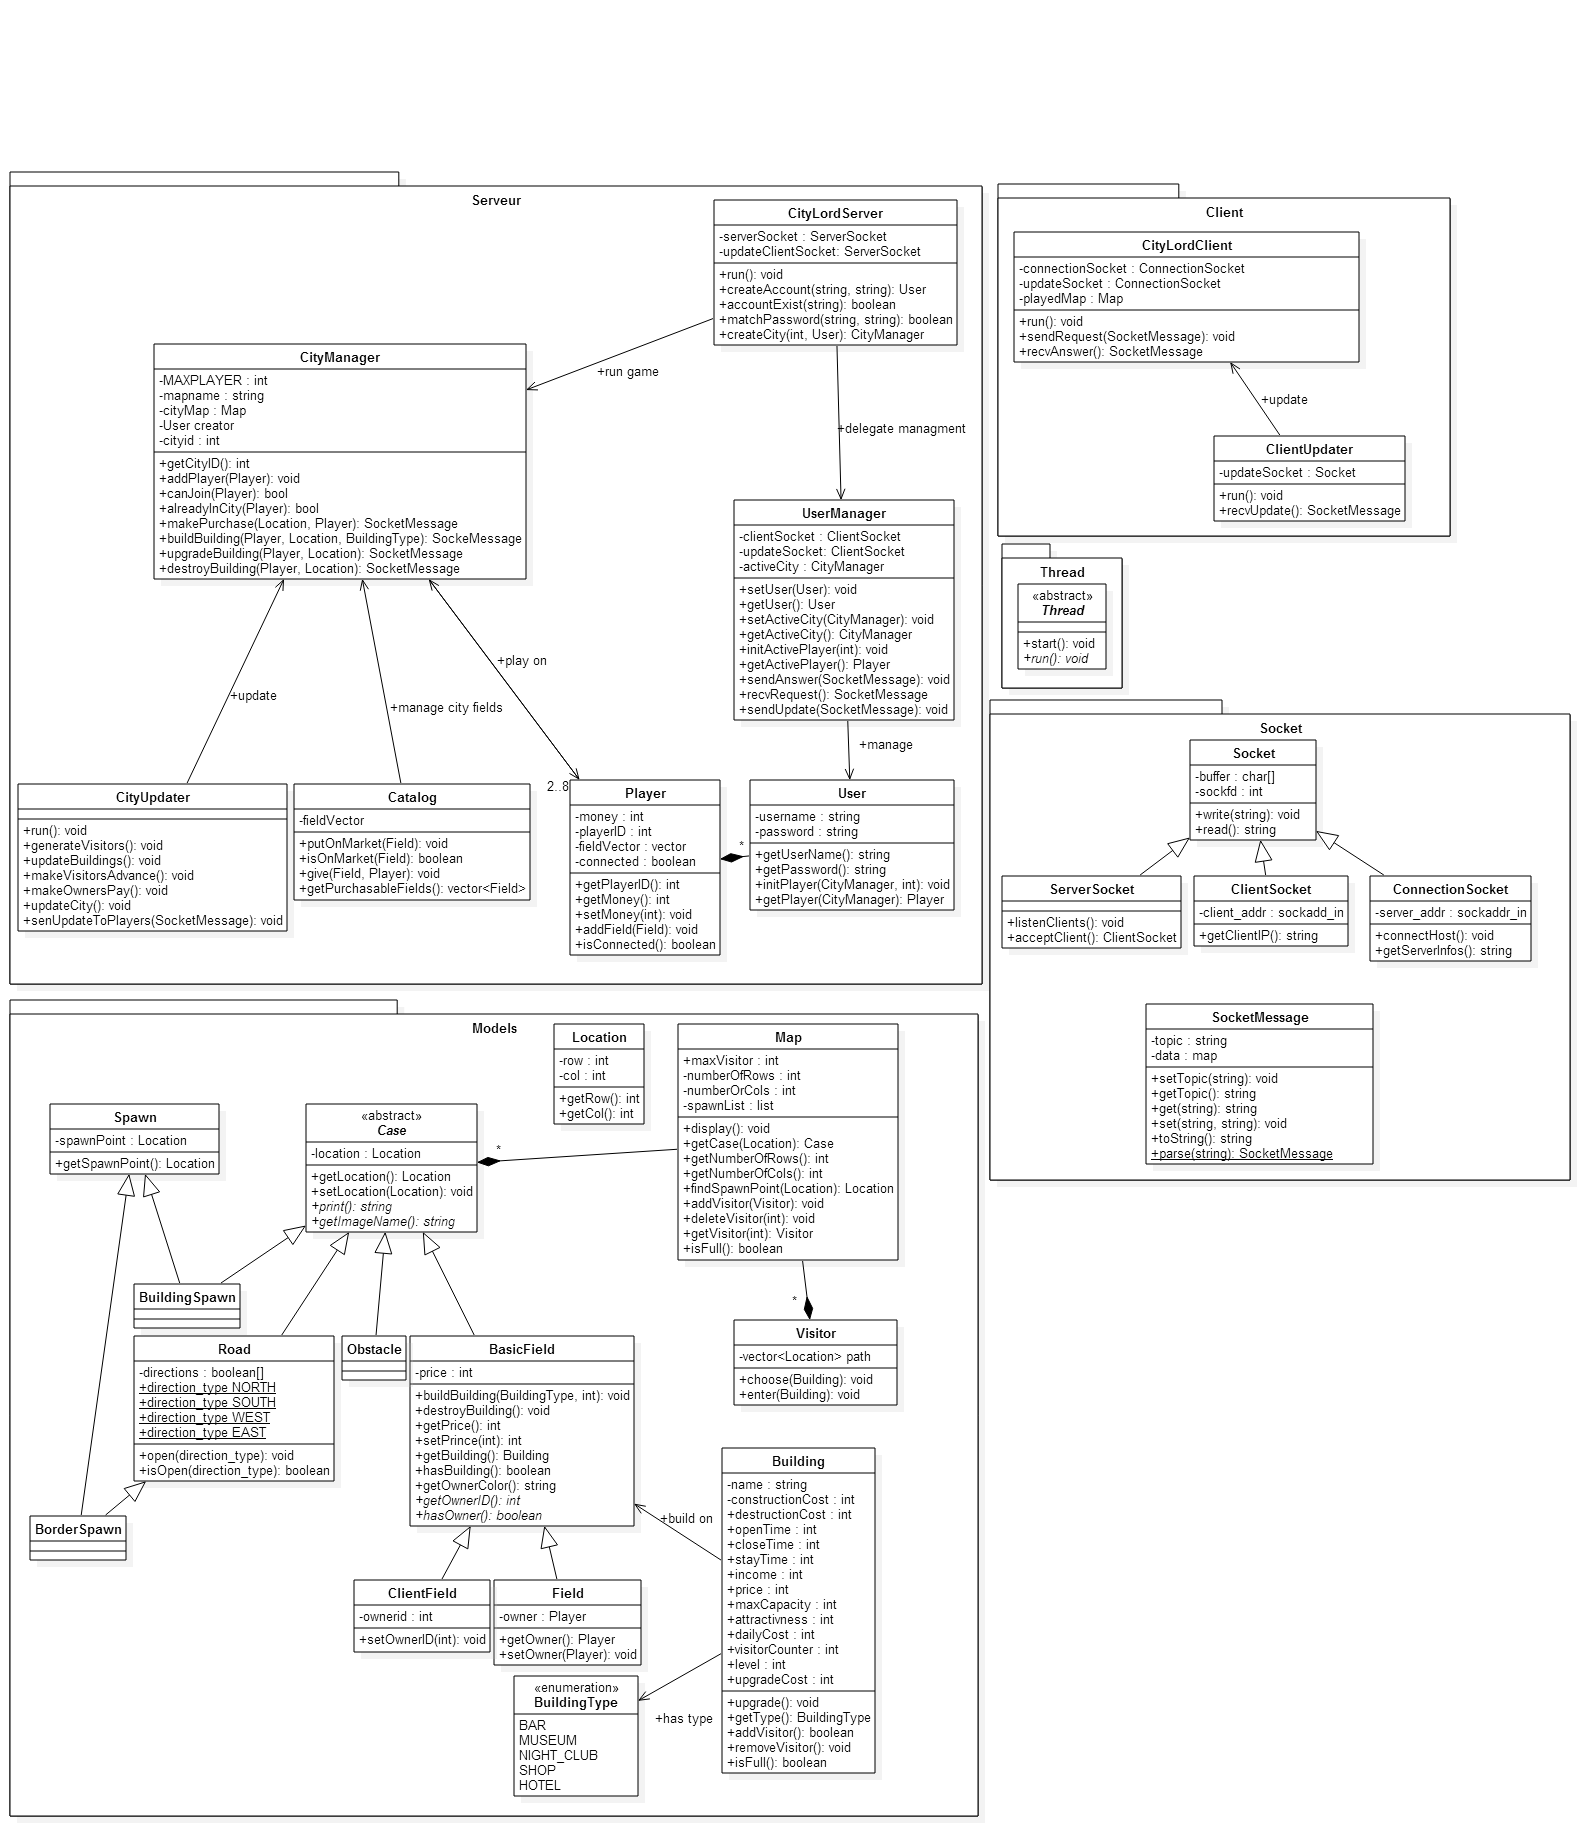
\includegraphics[width=550pt]{uml/classDiagrams/CD.png}
    }
    \caption{Diagramme de classe : Architecture du système}
\end{figure}
\begin{figure}[ht]
    \makebox[\linewidth]{
       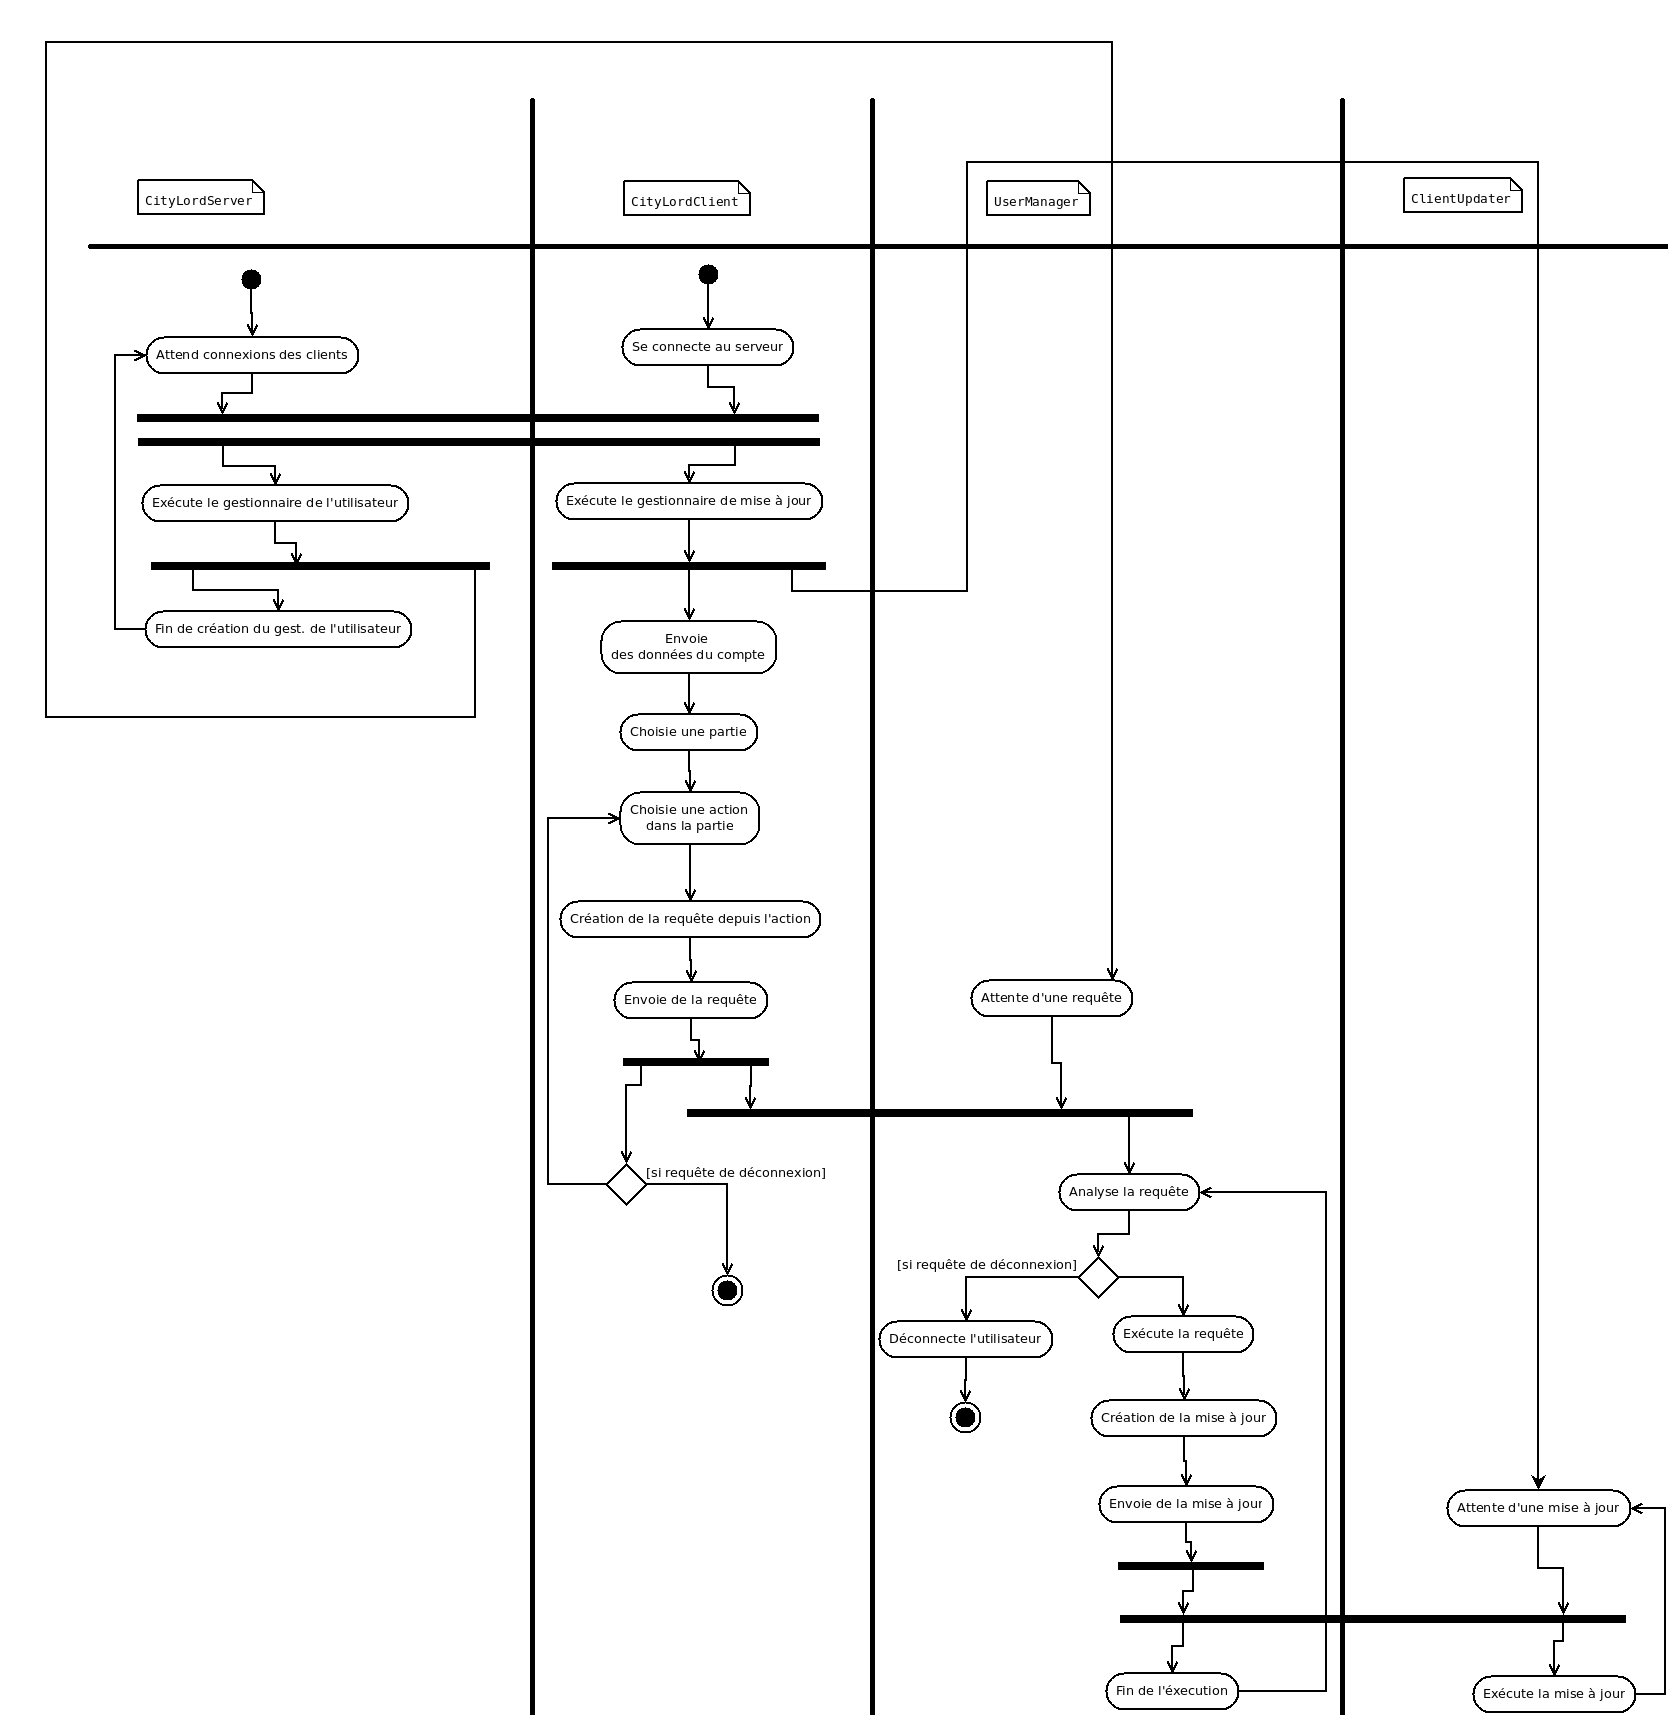
\includegraphics[width=550pt]{uml/activityDiagrams/activityDiagram.png}
    }
    \caption{Diagramme d'activité}
\end{figure}

\newpage
\subsection{Précision du diagramme de classe}
\paragraph{}
Une map est une matrice contenant des \textit{Case}. Une \textit{Case} est soit une parcelle (\textit{Field}) qui peut être achetée par un joueur où il pourra y construire des bâtiments, soit une route (\textit{Road}) permettant aux \textit{Visitors} de se déplacer, soit un obstacle (décoration  pour les joueurs), soit une zone d'entré pour les \textit{Visitors}. 

\newpage

\printindex


\end{document}
